\documentclass[11pt,a4paper]{article}
% Shared preamble for the Round 3 report (compiled from inside reports/)
\usepackage[utf8]{inputenc}
\usepackage[T1]{fontenc}
\usepackage{lmodern}
\usepackage[margin=2.2cm]{geometry}
\usepackage{graphicx}
\usepackage{xcolor}
\usepackage{booktabs}
\usepackage{enumitem}
\usepackage{titlesec}
\usepackage{fancyhdr}
\usepackage{tcolorbox}
\usepackage{float}
\usepackage{caption}
\usepackage{parskip}
\usepackage{array}
\usepackage{amsmath}
\usepackage{tabularx}
\usepackage{needspace}
\usepackage{etoolbox}
\usepackage{hyperref}

\graphicspath{{../images/}}

\definecolor{primary}{RGB}{44,62,80}
\definecolor{accent}{RGB}{52,152,219}
\definecolor{insightbg}{RGB}{235,245,255}
\definecolor{bodytext}{RGB}{50,50,50}

\hypersetup{colorlinks=true, linkcolor=accent, urlcolor=accent,
  pdfauthor={Saanvi Grover, Aditya Sharma}}

\titleformat{\section}{\Large\bfseries\color{primary}}{\thesection}{0.6em}{}[\color{accent}\titlerule]
\titleformat{\subsection}{\large\bfseries\color{primary}}{\thesubsection}{0.6em}{}
\titleformat{\subsubsection}{\normalsize\bfseries\color{primary}}{}{0em}{}

% Keep a heading with the text that follows it: reserve space before every heading,
% and forbid breaking immediately after one.
% A heading is often followed by a subheading and a table, so reserve generously.
\pretocmd{\section}{\Needspace*{10\baselineskip}}{}{}
\pretocmd{\subsection}{\Needspace*{7\baselineskip}}{}{}
\pretocmd{\subsubsection}{\Needspace*{5\baselineskip}}{}{}
\titlespacing*{\section}{0pt}{3.2ex plus 1ex minus .2ex}{1.6ex plus .2ex}
\titlespacing*{\subsection}{0pt}{2.6ex plus 1ex minus .2ex}{1.2ex plus .2ex}

% No single lines stranded at the top or bottom of a page
\clubpenalty=10000
\widowpenalty=10000
\displaywidowpenalty=10000
\brokenpenalty=10000

% Tables and figures stay near their text rather than drifting to the next page
\setlength{\floatsep}{10pt plus 2pt minus 2pt}
\setlength{\textfloatsep}{12pt plus 2pt minus 2pt}
\setlength{\intextsep}{10pt plus 2pt minus 2pt}
\renewcommand{\topfraction}{0.9}
\renewcommand{\bottomfraction}{0.8}
\renewcommand{\textfraction}{0.08}
\renewcommand{\floatpagefraction}{0.75}

\pagestyle{fancy}
\fancyhf{}
\fancyfoot[C]{\thepage}
\renewcommand{\headrulewidth}{0pt}

\newtcolorbox{insightbox}[1][KEY FINDING]{
  colback=insightbg, colframe=accent, boxrule=0.5pt, arc=2pt,
  left=8pt, right=8pt, top=6pt, bottom=6pt,
  fonttitle=\bfseries\small, coltitle=white, title=#1,
  before skip=8pt, after skip=8pt
}

\newcommand{\entropytitle}[2]{%
\begin{titlepage}
\centering
\vspace*{3cm}
{\Huge\bfseries\color{primary} #1\par}
\vspace{0.6cm}
{\Large\color{gray} #2\par}
\vspace{1.2cm}
{\color{accent}\rule{9cm}{1pt}\par}
\vspace{1.2cm}
{\large\color{gray} Round 3: Signal Tracking\par}
\vspace{1.4cm}
{\large
\begin{tabular}{rl}
\textbf{Competition:} & Data Vortex $|$ AARUUSH'26 \\
\textbf{Theme:} & Rebuilding the Social Engine \\
\textbf{Team:} & Entropy \\
\textbf{Members:} & Saanvi Grover \& Aditya Sharma \\[0.4cm]
\textbf{Assigned topic:} & Public Reaction to a Major Software Update \\
\textbf{Event tracked:} & iOS 27 / iPadOS 27 / macOS 27 release \\
\textbf{Comparison:} & Android 17 release \\
\end{tabular}
\par}
\vfill
\end{titlepage}
}

\hypersetup{pdftitle={Round 3 Analytical Report -- Team Entropy}}

\usepackage{url}
\begin{document}
\color{bodytext}
\entropytitle{Analytical Report}{Public reaction to the iOS 27 software update}

\section*{Executive summary}
\addcontentsline{toc}{section}{Executive summary}

We tracked public reaction to the \textbf{iOS 27 / iPadOS 27 / macOS 27} release (14 September 2026), using \textbf{Android 17} (18 September) as a comparison release. A purpose-written collector gathered \textbf{5,498 posts and comments} from Reddit, Hacker News, Mastodon and Lemmy across a 295-hour window in two snapshots; \textbf{1,403} of them, written by \textbf{1,132 distinct authors}, explicitly mention a tracked release and form the analysis set. Every post was scored with the \textbf{Round 2 sentiment ensemble}, reused without retraining.

\begin{insightbox}[HEADLINE]
The launch was not greeted badly -- it was greeted indifferently, and then soured. Net sentiment (share positive minus share negative) ran at \textbf{+0.05} before release (95\% CI $[-0.05, +0.15]$, so the baseline is \emph{not} measurably positive -- it is indistinguishable from neutral), \textbf{$-$0.12} in the first 24 hours, and \textbf{$-$0.37} after three days. The \emph{levels} at the start are uncertain; the \emph{decline} is not. Relative to baseline the drop reaches \textbf{0.43} (95\% CI $[0.31, 0.54]$) by day three, it is statistically significant at every pre-specified comparison, it survives holding the platform fixed, and it is not the work of a handful of accounts: \textbf{562 negative posts come from \textbf{521} distinct authors}. What people complain about is not the redesign but reliability: \textbf{bugs and crashes score $-$0.67} and \textbf{notifications $-$0.61}, while the visual redesign is the \emph{least} negative theme at $-$0.10. The single loudest moment of the window belongs to the comparison release: a Hacker News thread about \textbf{Android 17} withholding APIs from AOSP drew 1,135 points and an engagement spike \textbf{183 standard deviations} above baseline.
\end{insightbox}

\begin{table}[H]
\centering\small
\begin{tabular}{@{}lll@{}}
\toprule
\textbf{Rulebook requirement} & \textbf{Delivered} & \textbf{Section} \\
\midrule
At least 2 sentiment shifts & 3 significant shifts (2 pre-specified, 1 detected) & 4.3, 4.4 \\
At least 1 engagement spike & 44 spike hours; 3 analysed in depth & 5 \\
Key discussion topics / entities & 5 entities, 8 themes, 6 unsupervised topics & 6 \\
Reasons behind observed changes & 5 triggers evidenced by news and named posts & 7 \\
\bottomrule
\end{tabular}
\end{table}

\section{Data collection method}

\subsection{Sources and endpoints}

Collection is performed by \texttt{Entropy\_collect\_data.py}, a standalone Python script that uses only public, read-only endpoints and \textbf{no API keys}.

\begin{table}[H]
\centering\footnotesize
\begin{tabular}{@{}llll@{}}
\toprule
\textbf{Source} & \textbf{Endpoint} & \textbf{Collected} & \textbf{Engagement field} \\
\midrule
Reddit & \texttt{/r/*/search.rss}, \texttt{/comments/*.rss} & 1,054 posts, 688 comments & not exposed by RSS \\
Hacker News & \texttt{hn.algolia.com/api/v1/search} & 126 stories, 1,919 comments & points, comment count \\
Mastodon & \texttt{\{instance\}/api/v1/timelines/tag/} & 1,594 posts & favourites + boosts \\
Lemmy & \texttt{\{instance\}/api/v3/search} & 88 posts, 29 comments & score, comment count \\
Google News & \texttt{news.google.com/rss/search} & 390 articles & n/a (event timeline) \\
\bottomrule
\end{tabular}
\caption{Five public sources. Google News is used only to date real-world events and is never counted as public reaction.}
\end{table}

Queries covered \texttt{iOS 27}, \texttt{iPadOS 27}, \texttt{macOS 27}, \texttt{Apple Intelligence} and \texttt{Android 17} across 9 subreddits, 4 Mastodon instances (17 hashtag timelines) and 3 Lemmy instances. Reddit was searched twice, by recency and by popularity, and the most-discussed threads were expanded comment by comment; Hacker News threads were expanded for the 20 most-commented stories, which is where long-form opinion lives.

\subsection{Three obstacles and how they were handled}

\begin{itemize}[leftmargin=*]
  \item \textbf{Reddit blocks anonymous JSON.} \texttt{api.reddit.com} returns HTTP 403 and \texttt{old.reddit.com/*.json} serves an interstitial page. The Atom (RSS) interface still works and is used instead. The cost is that \textbf{RSS does not expose scores}, so Reddit contributes text and timing but not engagement values.
  \item \textbf{Anonymous feeds are rate limited} to roughly one request per minute. Reddit therefore runs in a dedicated slow lane (45\,s between calls, exponential backoff on HTTP 429) while other sources run at 1.2\,s. Across both runs, 417 requests were issued and 31 failed after retries; every attempt is logged.
  \item \textbf{Popularity is invisible in RSS.} A first run picked threads by recency and recovered only 31 comments. Because a \texttt{sort=top} search returns posts in popularity order, the second run used that ordering to choose which threads to expand, raising Reddit comments to \textbf{688}.
\end{itemize}

\subsection{Structure, ethics and reproducibility}

Every record is normalised to one schema: \texttt{source}, \texttt{source\_detail}, \texttt{kind} (post or comment), \texttt{post\_id}, \texttt{parent\_id}, \texttt{created\_utc}, \texttt{title}, \texttt{text}, \texttt{author\_hash}, \texttt{score}, \texttt{n\_replies}, \texttt{url}, \texttt{query}, \texttt{lang}, \texttt{collected\_at}. \textbf{Author names are replaced by a salted SHA-256 hash}, so no personal identifiers are stored. A manifest records every query, counts and timings, and the full request log is stored gzipped beside the data.

\begin{table}[H]
\centering\small
\begin{tabular}{@{}lrlr@{}}
\toprule
\textbf{Stage} & \textbf{Rows} & \textbf{Analysis set by source} & \textbf{Posts} \\
\midrule
Fetched across two runs      & 16,010 & Reddit      & 718 \\
In window, de-duplicated     & 5,498  & Mastodon    & 513 \\
Mentions a tracked release   & 1,829  & Hacker News & 138 \\
\textbf{English analysis set}& \textbf{1,403} & Lemmy & 34 \\
\bottomrule
\end{tabular}
\caption{From raw collection to analysis set: 1,132 distinct authors, 1,250 posts and 153 comments.}
\end{table}

Two scripts produce everything in this report. \texttt{Entropy\_collect\_data.py} performs the collection described above; \texttt{Entropy\_03\_robustness\_checks.py} produces the period intervals, the author-concentration check, the VADER baseline, the alert replay and the inter-annotator figures in section 7, writing them to \texttt{outputs/Entropy\_round3\_robustness.json}. Both, together with the notebook, the annotation sheets and the consensus labels, are in the team repository at \url{https://github.com/SaiGrover/entropy-data-vortex}.

\section{Time window}

Collection covers \textbf{8 September 2026 01:10 UTC to 20 September 2026 10:44 UTC} (297.6 hours); the analysis set, being a subset, spans \textbf{03:48 UTC on 8 September} to the same end point (294.9 hours), and it is that figure the per-hour rates in this report are computed over. The window starts six days \emph{before} the iOS 27 release so that a pre-launch baseline exists: without one, a negative reading after launch cannot be distinguished from a community that is negative all the time. All timestamps come from each platform's own metadata and are normalised to UTC.

The window is divided into four periods: pre-launch, the first 24 hours, 24--72 hours, and beyond. Two release moments anchor it: \textbf{iOS 27 on 14 September $\approx$17:00 UTC} and \textbf{Android 17 on 18 September}.

\begin{figure}[H]\centering
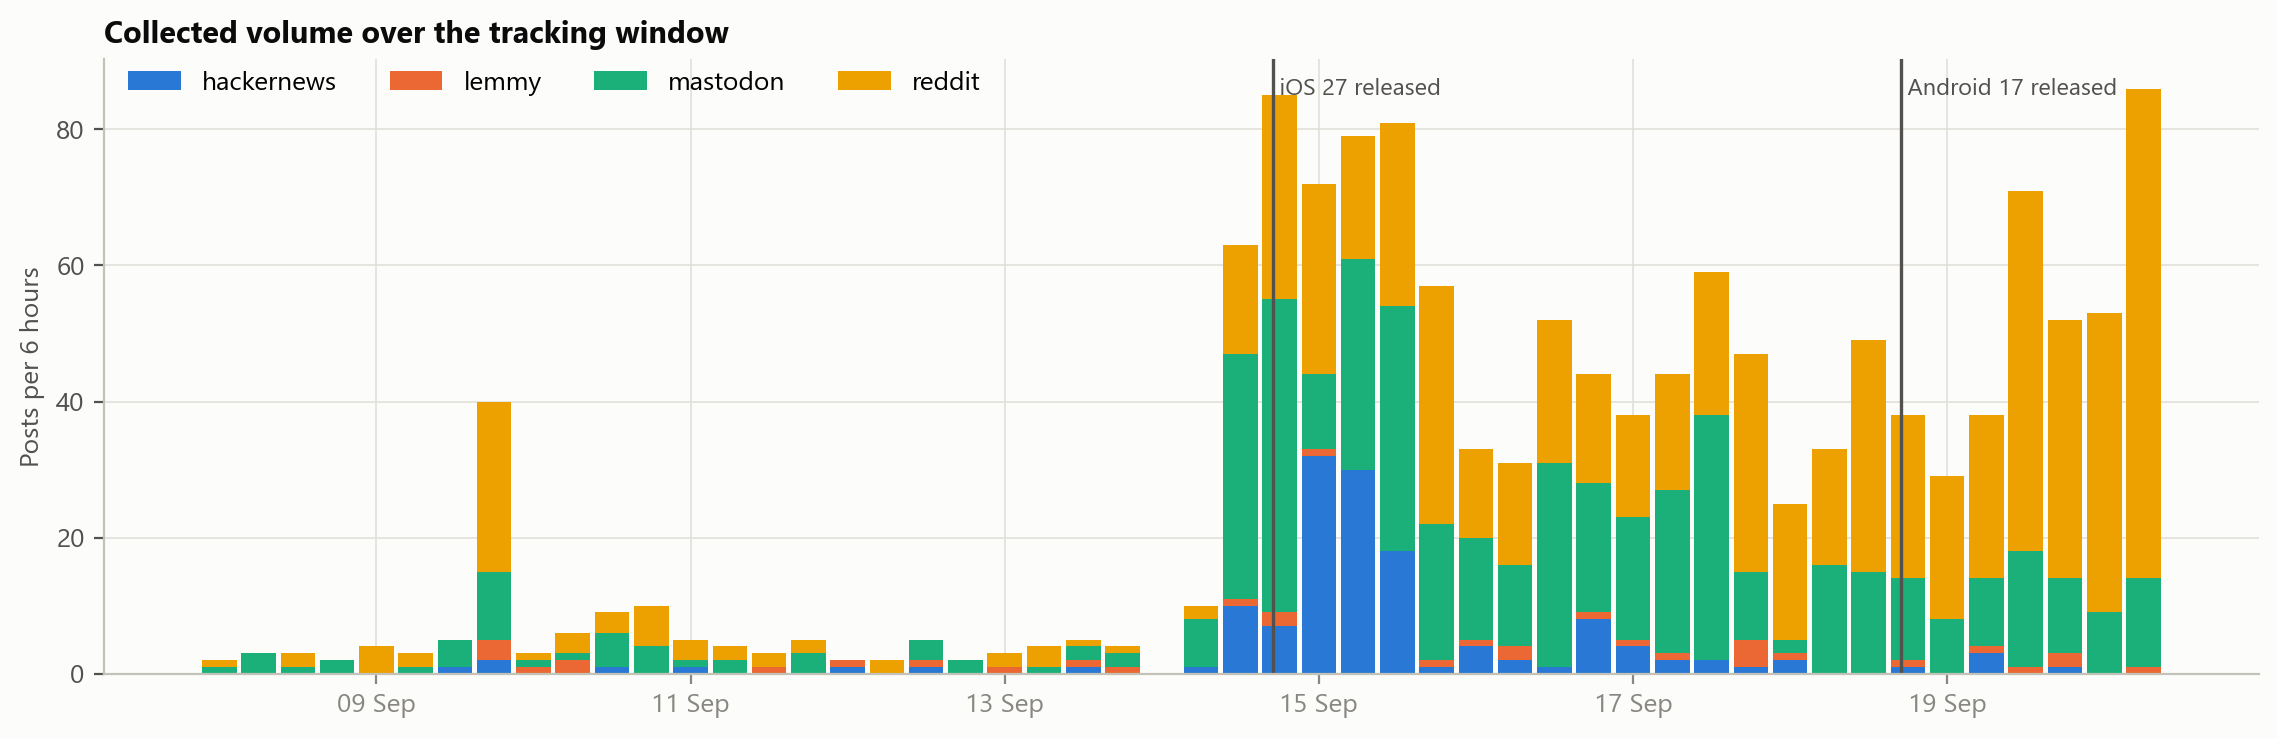
\includegraphics[width=\textwidth]{Entropy_r3_volume_timeline.png}
\caption{Collected volume per 6 hours by platform. Activity is minimal before the release, jumps at launch, and stays elevated.}
\end{figure}

\section{Sentiment analysis}

\subsection{Applying the Round 2 model}

The Round 2 artefact is loaded exactly as trained: a weighted ensemble of TF-IDF logistic regression (0.25), MiniLM sentence embeddings with logistic regression (0.20) and three fine-tuned MiniLM seeds (0.55). Three practical details were handled rather than ignored.

\begin{itemize}[leftmargin=*]
  \item \textbf{Library compatibility.} The pickles were written by a newer scikit-learn than the one installed, which no longer sets \texttt{multi\_class} on \texttt{LogisticRegression}. The attribute is restored to the trained value (\texttt{multinomial}) instead of retraining.
  \item \textbf{Operating point.} The artefact carries a validation-selected bias of 1.05 on the Neutral class. The saved \texttt{predict()} applies it but \texttt{predict\_proba()} does not, so scoring through \texttt{predict\_proba} would silently use a different operating point than Round 2 chose. The bias is applied here.
  \item \textbf{Truncation.} The fine-tuned component was trained on tweets with \texttt{max\_len}~=~50 tokens, but posts here have a median length of 74 tokens and \textbf{68\% exceed 50}. Scoring them directly would read only the opening of two thirds of the corpus, so long posts are split into overlapping 34-word windows and their probabilities averaged.
\end{itemize}

\subsection{How accurate is the model on this data?}

Round 2 reported macro-F1 0.723 on labelled tweets. To measure the model where it is actually used, \textbf{150 posts were drawn at random} (not stratified by prediction, which would flatter the estimate) and labelled by hand against a fixed rubric: Positive = approval or a favourable experience; Negative = complaint, bug report or criticism; Neutral = factual news, an announcement, or a question with no clear valence.

\begin{table}[H]
\centering\small
\begin{tabular}{@{}lrrr@{}}
\toprule
\textbf{Scorer} & \textbf{Macro-F1} & \textbf{Accuracy} & \textbf{Reference} \\
\midrule
VADER lexicon & 0.496 & --- & consensus \\
Round 2 ensemble, as-is (truncated) & 0.712 & --- & consensus \\
\textbf{Round 2 ensemble, chunked $+$ neutral bias (used)} & \textbf{0.699} & \textbf{0.707} & consensus \\
\addlinespace
Same model, against the first annotator alone & 0.666 & 0.687 & single \\
\bottomrule
\end{tabular}
\caption{In-domain validation against the 140-post two-annotator consensus (66 Negative, 39 Neutral, 35 Positive). The final row shows the same model scored against the original single annotator, for comparison.}
\end{table}

Two points deserve stating plainly. First, the model scores \textbf{0.699 macro-F1} against the consensus, which is close to the 0.666 measured against the first annotator alone -- the estimate is not an artefact of who labelled. Second, and less comfortably, \textbf{the two inference corrections are not measurably better than plain truncation on this evidence}: chunked scoring comes out -0.013 against as-is, with a 95\% interval of $[-0.071, +0.045]$ from a paired bootstrap, which includes zero. Against the first annotator's labels the corrections appeared to help by 0.034; against the consensus that ordering does not replicate. We keep the chunked configuration because its justification is structural rather than empirical -- truncation at 50 tokens discards text from 68\% of these posts, and a scorer should read the post it is scoring -- but we do not claim it raises accuracy here. Across a 400-post sample chunking changes \textbf{12\% of labels}. The residual difference from 0.723 is genuine domain shift: these posts are longer, more technical and more often questions than the tweets the model was trained on. The confusion matrix shows where the model is weakest -- 21 of 70 truly Negative posts are read as Neutral, and 14 of 65 Neutral posts as Positive -- so absolute sentiment levels should be read with more caution than \emph{changes} in them, which is what this report relies on.

Across the analysis set the distribution is \textbf{40.1\% Negative, 40.9\% Neutral, 19.0\% Positive} (mean confidence 0.57).

\subsection{Two pre-specified shifts}

Rather than scanning every boundary and reporting whatever looked largest, three comparisons were fixed in advance and corrected with Holm's method.

\begin{table}[H]
\centering\small
\begin{tabular}{@{}lrrrrll@{}}
\toprule
\textbf{Period} & \textbf{n} & \textbf{Positive} & \textbf{Negative} & \textbf{Net} & \textbf{95\% CI} & \textbf{Change vs previous} \\
\midrule
Pre-launch (8--14 Sep) & 171 & 25.1\% & 19.9\% & $+0.05$\,$^{\dagger}$ & $[-0.05, +0.15]$ & --- \\
Launch $+$0--24h & 330 & 24.5\% & 36.7\% & $-0.12$ & $[-0.20, -0.04]$ & $-0.17$, Holm $p = 0.0002$ \\
Settling $+$24--72h & 355 & 22.8\% & 39.7\% & $-0.17$ & $[-0.25, -0.09]$ & $-0.05$, not significant \\
Later ($+$72h onward) & 547 & 11.3\% & 48.6\% & $-0.37$ & $[-0.43, -0.32]$ & $-0.20$, Holm $p = 0.00001$ \\
\bottomrule
\end{tabular}
\caption{Net sentiment by period, with 95\% bootstrap intervals from 8{,}000 multinomial resamples of each period's class counts. $\dagger$ marks an interval that includes zero: the pre-launch baseline is indistinguishable from neutral, so the decline is a fall from indifference rather than from approval. The first and third comparisons remain significant after Holm correction.}
\end{table}

\begin{figure}[H]
\centering
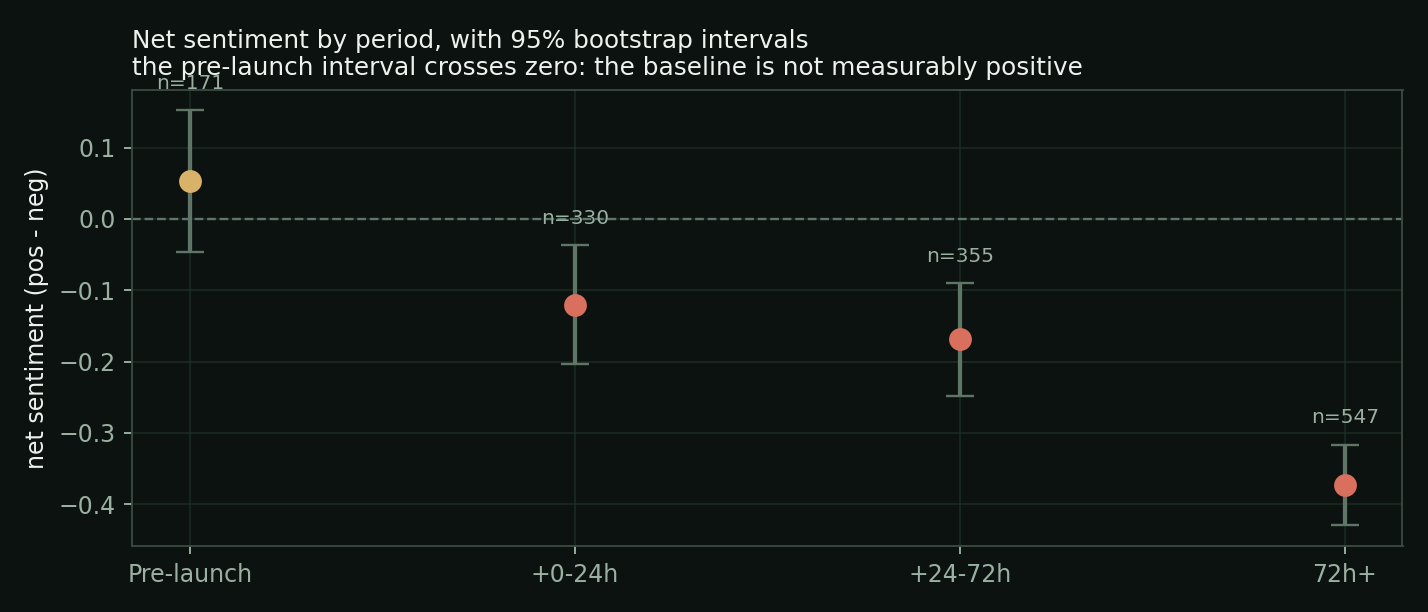
\includegraphics[width=0.94\textwidth]{Entropy_r3_fig8_periods_ci.png}
\caption{The same four periods as intervals rather than points. Only the pre-launch interval crosses zero, and it is also the thinnest period at $n=171$.}
\end{figure}

\subsection{One detected shift}

Independently, consecutive 12-hour bins (minimum 40 posts) were compared pairwise with two-proportion z-tests and Holm correction across all 24 boundaries. One survives, and it is sharp: at \textbf{15 September 00:00 UTC} net sentiment falls from $+0.16$ to $-0.26$ ($n = 148 \to 151$, Holm $p < 0.0001$) -- the first full night after release, when the update reached ordinary users rather than enthusiasts.

\begin{figure}[H]\centering
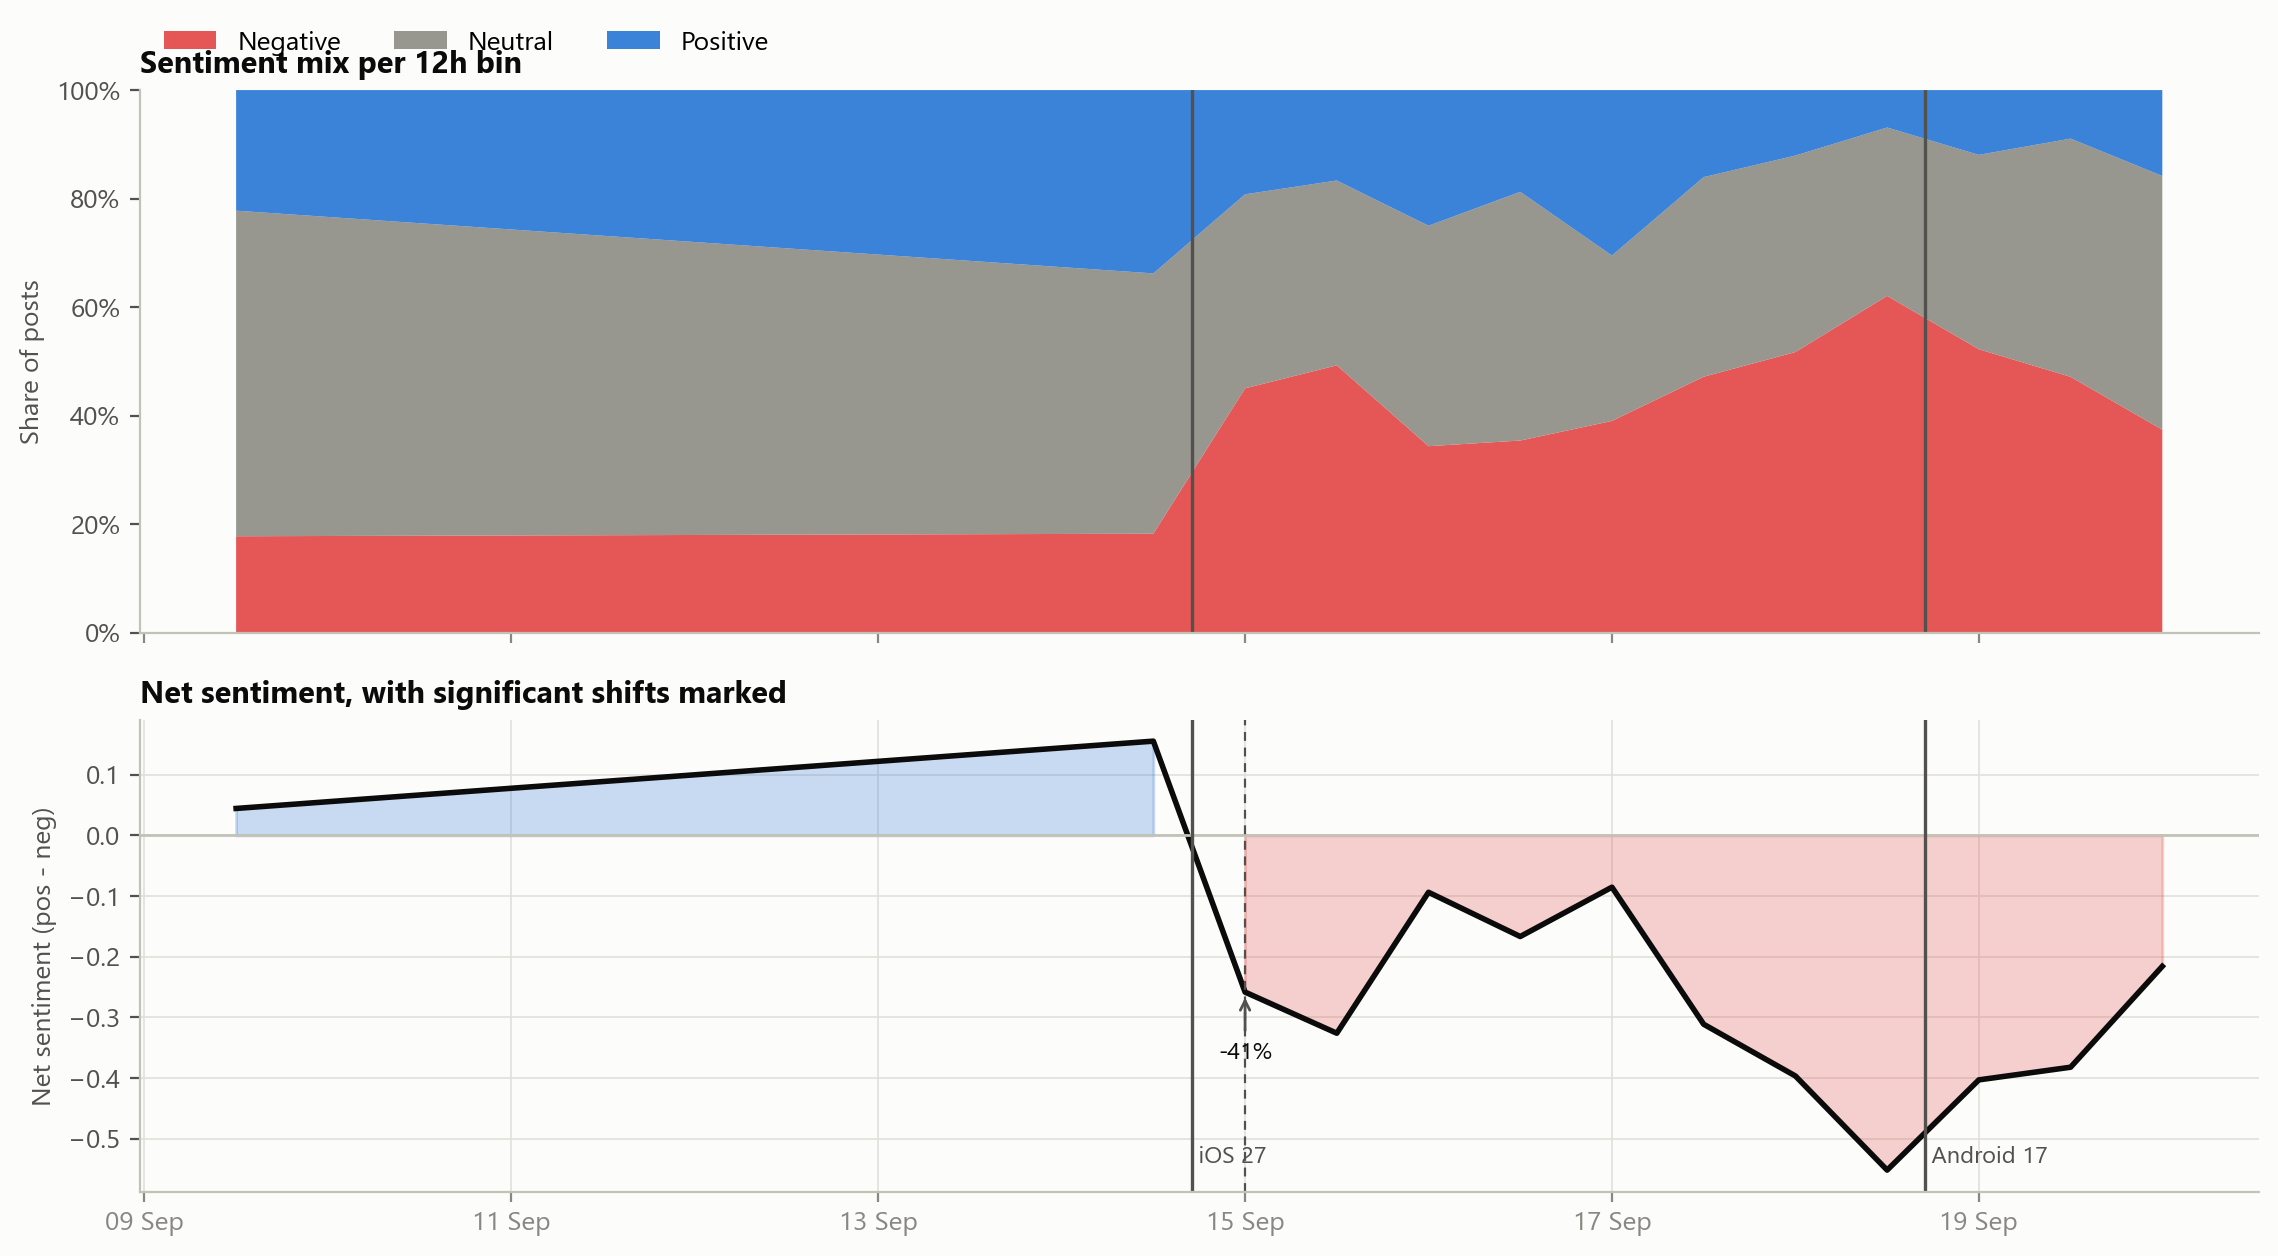
\includegraphics[width=\textwidth]{Entropy_r3_sentiment_timeline.png}
\caption{Sentiment mix per 12-hour bin (top) and net sentiment with the significant shift marked (bottom).}
\end{figure}

\subsection{Is the decline real, or a change in who we sampled?}

Reddit is the most negative platform here and its share grows across the window, so the decline could in principle be an artefact of sampling. Holding the platform fixed removes that objection: on \textbf{Mastodon alone}, where coverage is good at both ends of the window, net sentiment falls from $+0.43$ (n = 70) to $-0.17$ (n = 146). Positive posts drop from 57.1\% to 24.0\% ($p = 0.0002$) and negative posts rise from 14.3\% to 41.1\% ($p = 3.6 \times 10^{-8}$).

\begin{insightbox}
The decline is real, but the raw figure overstates it. A monitoring system that reports one global sentiment line will mislead whenever its source mix changes; baselines must be computed per platform. Our own headline number ($-0.37$) is part sentiment and part sampling, and only the within-platform comparison separates the two.
\end{insightbox}

\section{Activity analysis}

Hourly volume and hourly engagement were each scored with a robust z-score against a trailing 48-hour median and median absolute deviation, falling back to a trailing standard deviation when the baseline is flat. 44 hours exceed $z > 3$ on at least one measure.

\begin{table}[H]
\centering\small
\begin{tabular}{@{}llrrl@{}}
\toprule
\textbf{Hour (UTC)} & \textbf{Type} & \textbf{Posts} & \textbf{Engagement} & \textbf{Robust z} \\
\midrule
14 Sep 17:00 & volume + engagement & 36 & 851   & $z_{\text{posts}} = 97.1$, $z_{\text{eng}} = 56.0$ \\
18 Sep 19:00 & engagement          & 13 & 1,157 & $z_{\text{eng}} = 183.0$ \\
09 Sep 18:00 & volume + engagement & 14 & 16    & $z_{\text{posts}} = 14.9$ \\
18 Sep 04:00 & engagement          & 3  & 156   & $z_{\text{eng}} = 21.4$ \\
\bottomrule
\end{tabular}
\caption{The largest spikes. The release hour is the volume peak; the largest engagement peak belongs to Android 17.}
\end{table}

\begin{figure}[H]\centering
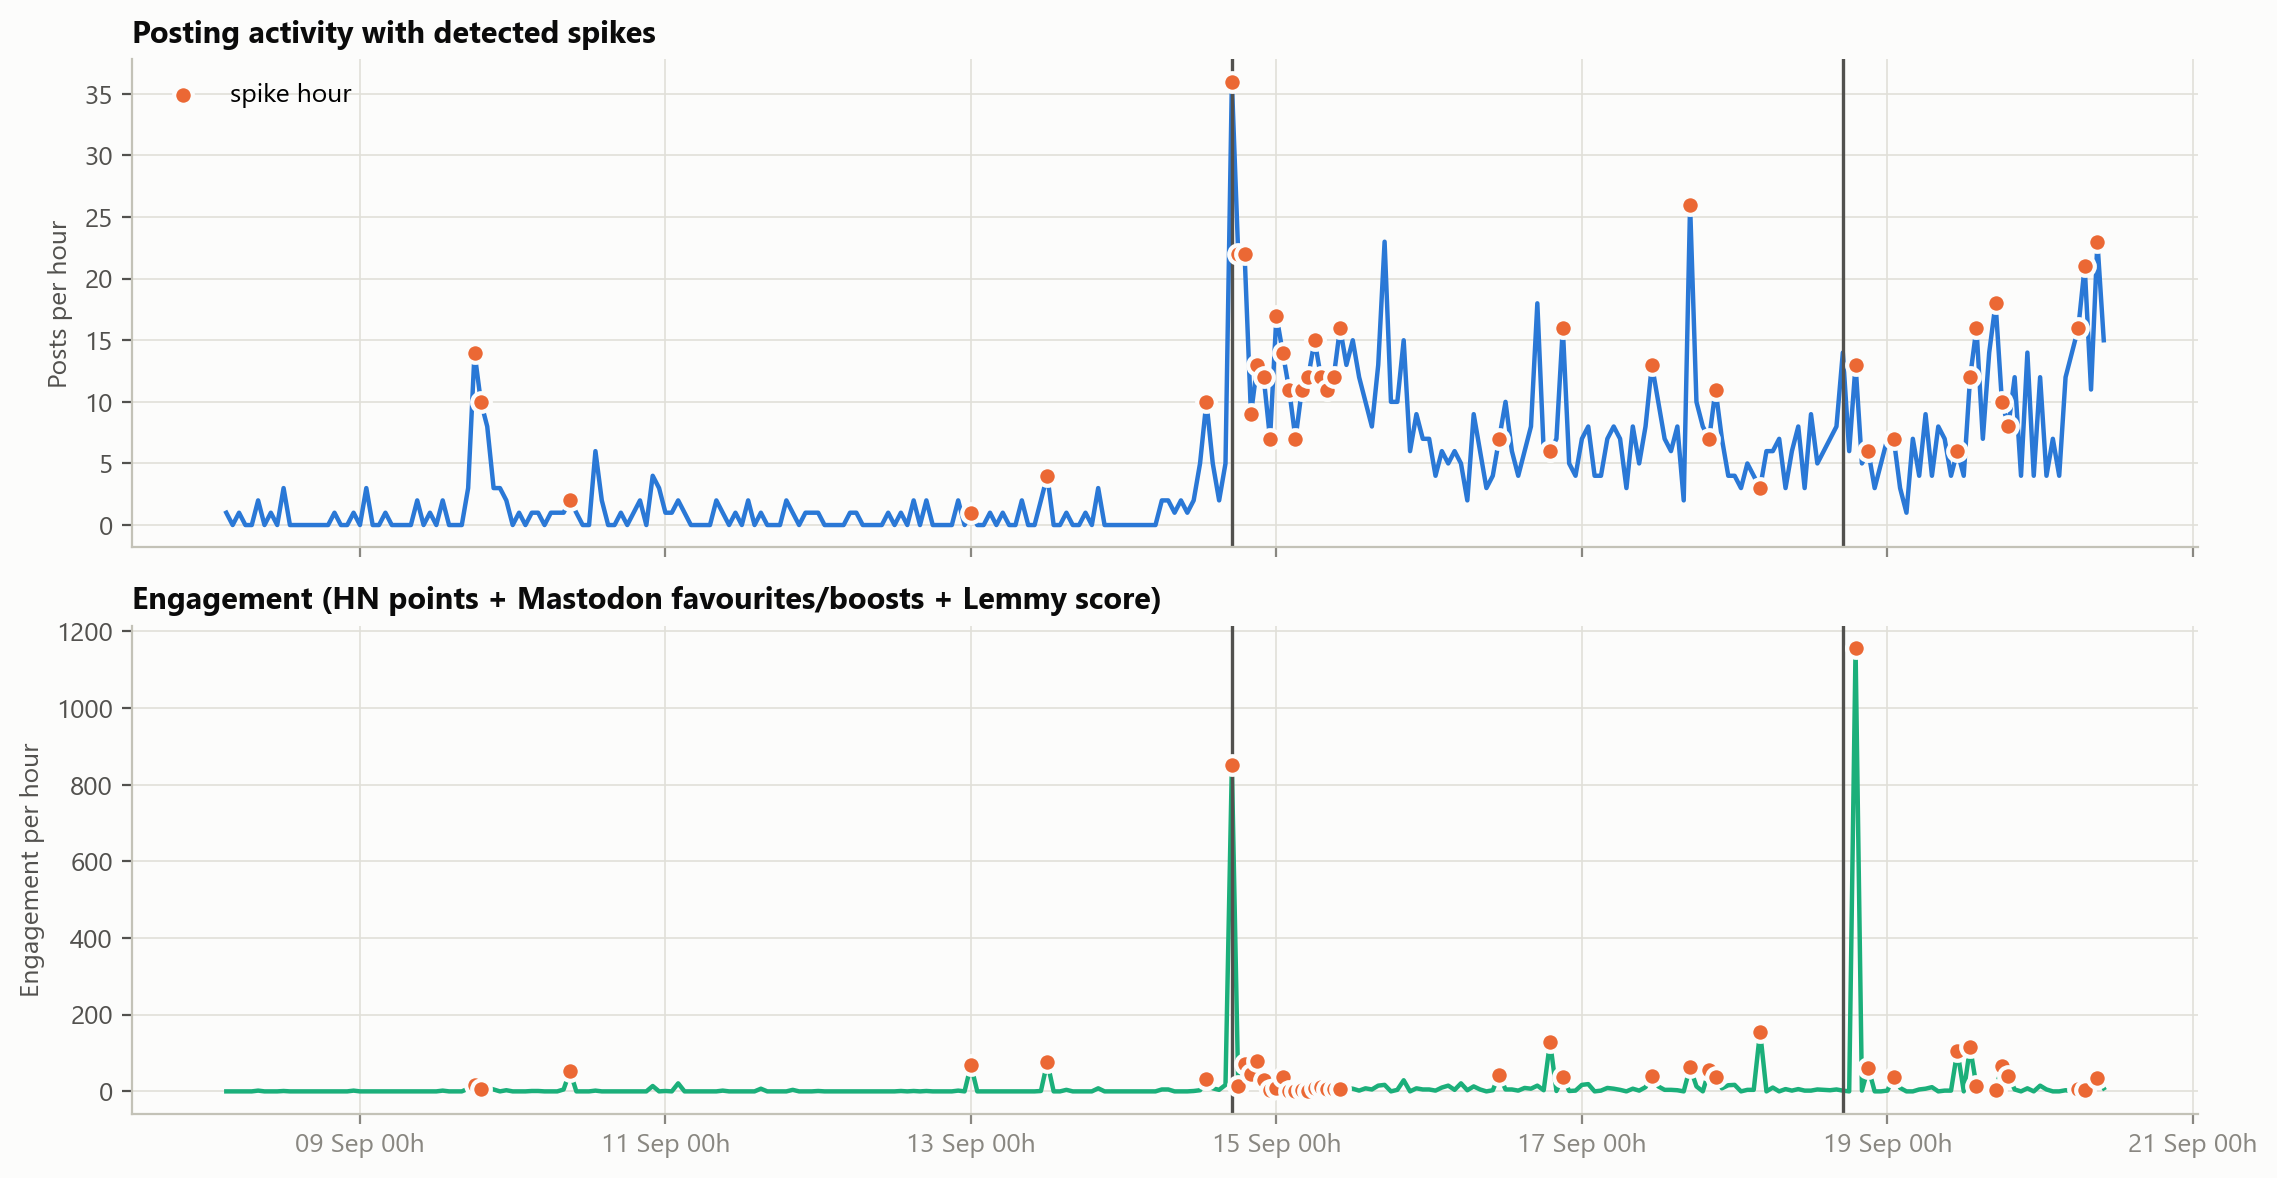
\includegraphics[width=\textwidth]{Entropy_r3_activity_spikes.png}
\caption{Posting activity (top) and engagement (bottom) per hour, with detected spikes marked.}
\end{figure}

Two structural points follow. First, \textbf{volume and engagement peak at different moments}: the release produced the most posts, but a single Hacker News thread four days later produced far more engagement from only 13 posts. Second, posting stays elevated for the rest of the window instead of decaying, which is what makes the later sentiment reading meaningful rather than the noise of a few stragglers.

\section{Topic and entity analysis}

\subsection{Entities and themes}

\begin{table}[H]
\centering\small
\begin{tabular}{@{}lrr|lrr@{}}
\toprule
\textbf{Entity} & \textbf{Mentions} & \textbf{Net} & \textbf{Theme} & \textbf{Mentions} & \textbf{Net} \\
\midrule
iOS 27             & 784 & $-0.16$ & Bugs / crashes           & 181 & $-0.67$ \\
macOS 27           & 378 & $-0.22$ & Notifications            & 54  & $-0.61$ \\
Apple Intelligence & 344 & $-0.22$ & Privacy                  & 50  & $-0.42$ \\
Android 17         & 127 & $-0.19$ & Install / update process & 149 & $-0.30$ \\
iPadOS 27          & 83  & $-0.08$ & Siri / assistant         & 279 & $-0.27$ \\
                   &     &         & Performance              & 115 & $-0.25$ \\
                   &     &         & Battery                  & 59  & $-0.15$ \\
                   &     &         & UI / design              & 173 & $-0.10$ \\
\bottomrule
\end{tabular}
\caption{Net sentiment per entity and theme. Every theme is net negative, but they are not equally negative.}
\end{table}

The ranking is the finding. Reliability complaints (bugs, notifications, installation) sit two to six times further below zero than the visual redesign, which is the \emph{least} negative theme at $-0.10$ despite being the most visible change in the release. Privacy at $-0.42$ is driven by the Apple Intelligence opt-in and data-training questions rather than by the operating system itself.

\begin{figure}[H]\centering
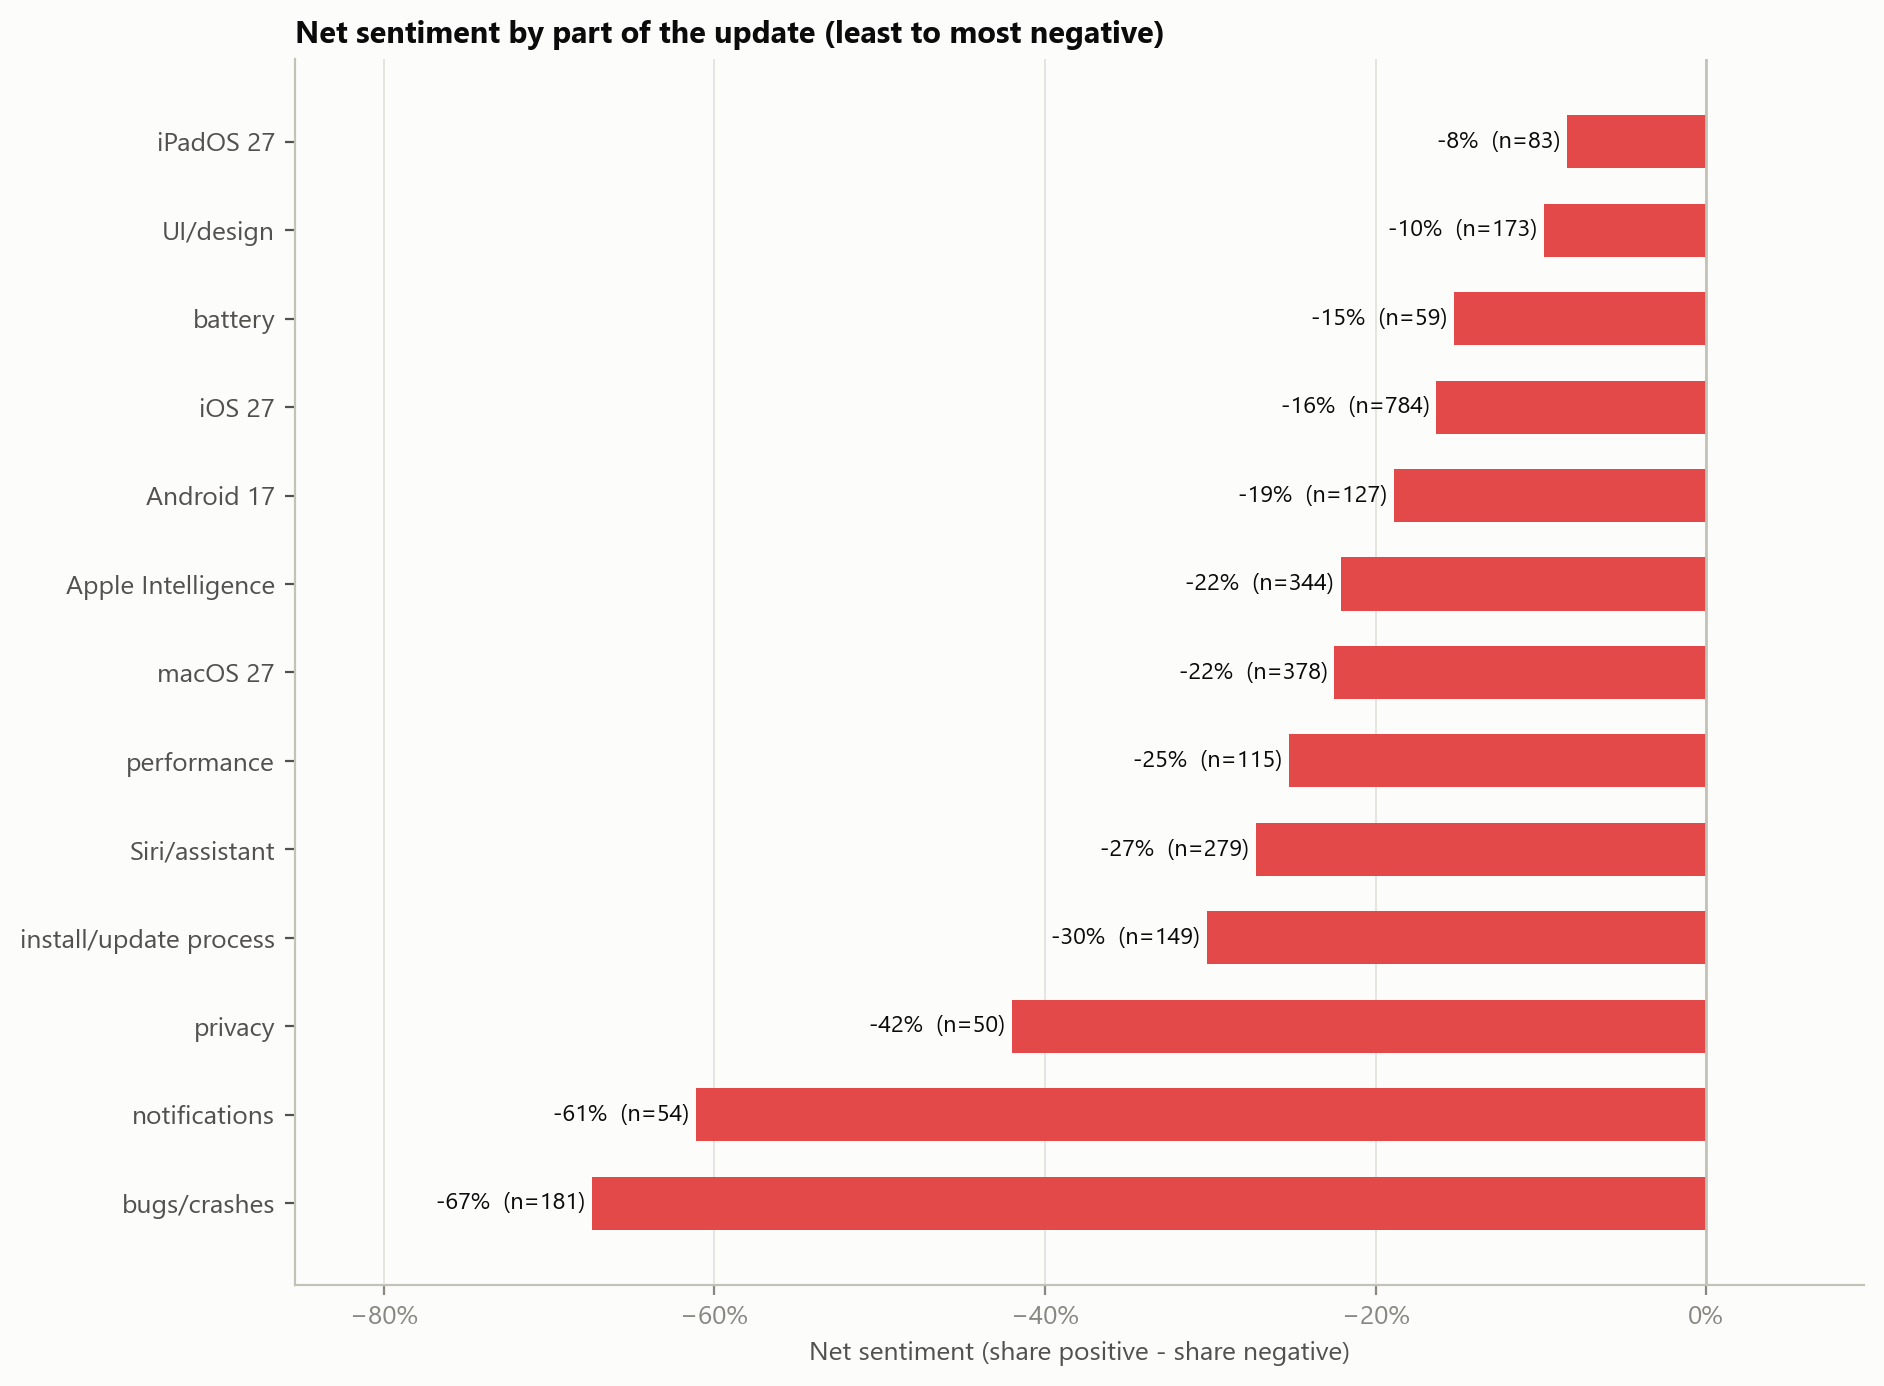
\includegraphics[width=0.95\textwidth]{Entropy_r3_entity_sentiment.png}
\caption{What people disliked most. Reliability dominates; the redesign is comparatively mild.}
\end{figure}

\subsection{Which words separate positive from negative}

Using log-odds ratios with an informative Dirichlet prior (Monroe et al., 2008), the most positive-leaning terms are \emph{new}, \emph{new features}, \emph{improvements}, \emph{health}, \emph{galaxy}; the most negative-leaning are \emph{issue}, \emph{problem}, \emph{bug}, \emph{fix}, \emph{tried}, \emph{storage}. The negative vocabulary is the vocabulary of \textbf{troubleshooting}: people are not debating taste, they are reporting things that stopped working.

\subsection{Unsupervised topics}

Non-negative matrix factorisation (6 topics) over the analysis set:

\begin{table}[H]
\centering\small
\begin{tabular}{@{}rlrr@{}}
\toprule
\textbf{\#} & \textbf{Leading terms} & \textbf{Posts} & \textbf{Net} \\
\midrule
0 & ios, ios 27, iphone, ios 26, update & 392 & $-0.31$ \\
1 & macos, macos 27, golden gate        & 299 & $-0.28$ \\
5 & ios27, app, macos27, new, apps      & 233 & $+0.13$ \\
3 & siri, ai, siri ai, new siri         & 207 & $-0.34$ \\
2 & android, android 17, pixel, qpr1    & 141 & $-0.22$ \\
4 & apple, intelligence, feature        & 131 & $-0.13$ \\
\bottomrule
\end{tabular}
\caption{The Siri/AI cluster is the most negative; developer and app-ecosystem talk is the only positive cluster.}
\end{table}

\begin{figure}[H]\centering
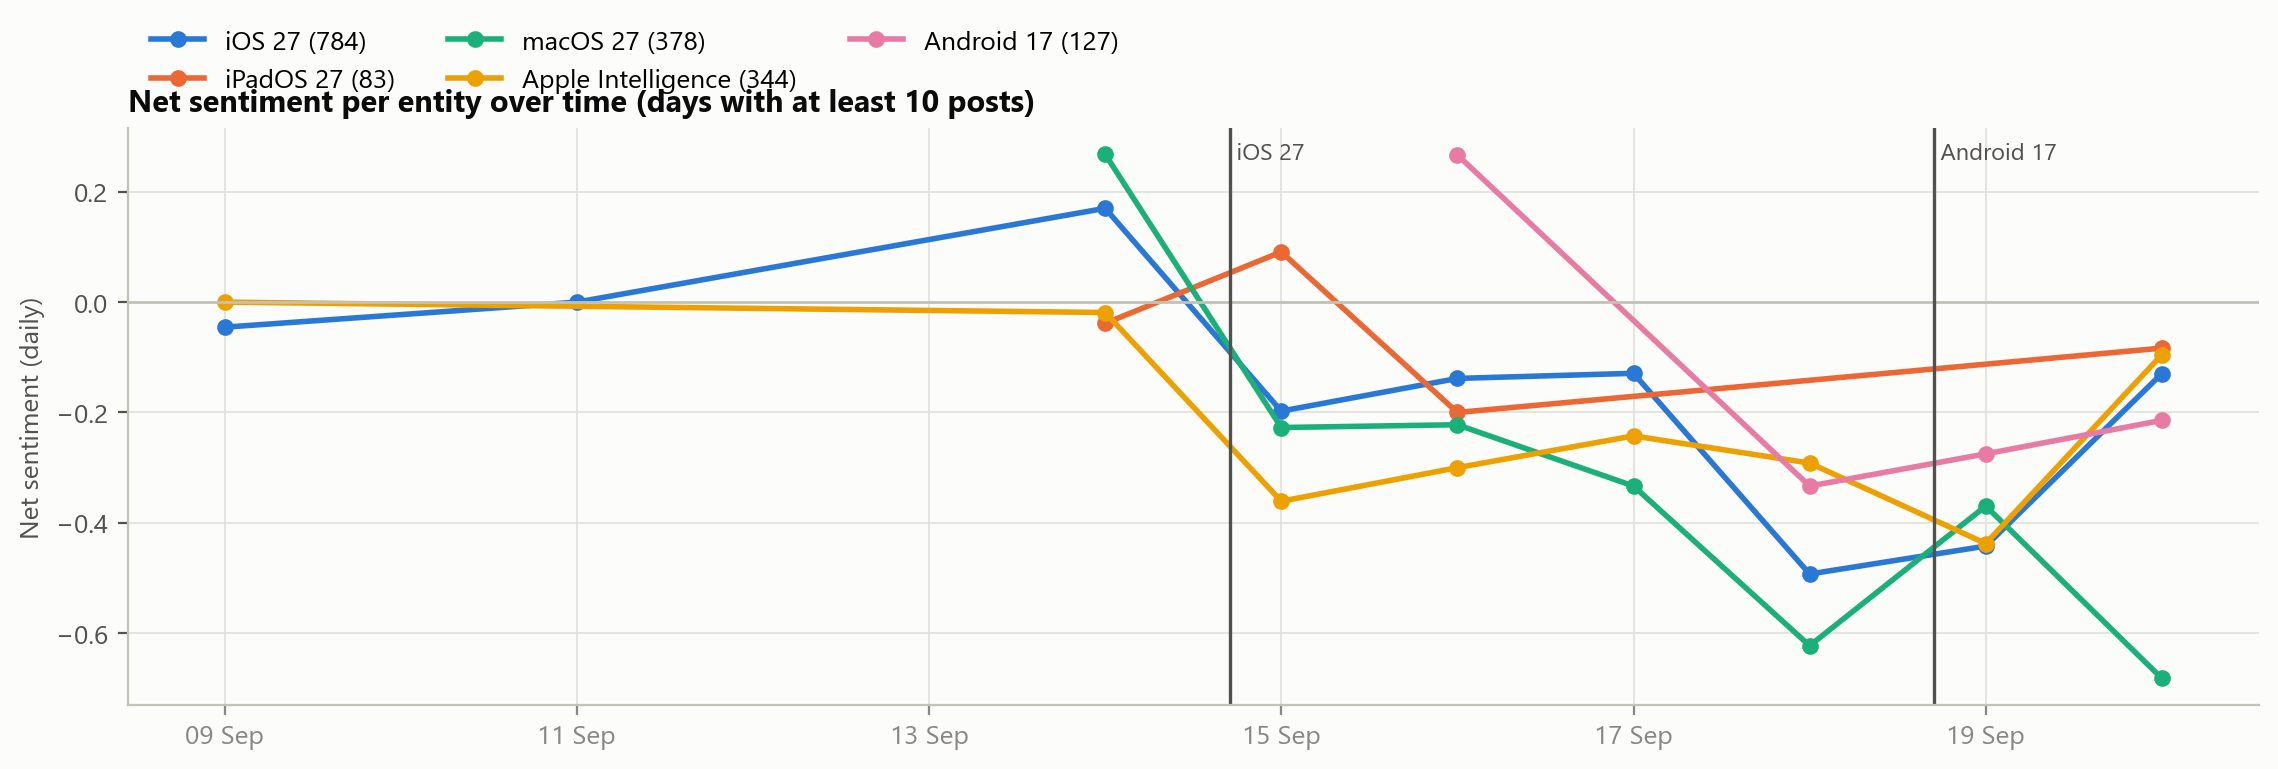
\includegraphics[width=\textwidth]{Entropy_r3_entity_sentiment_timeline.png}
\caption{Net sentiment per entity over time. Apple Intelligence and macOS 27 deteriorate after launch while iPadOS 27 stays flat.}
\end{figure}

\section{Trigger explanations}

Each spike and shift was matched against two independent kinds of evidence: news articles published in the same window, and the most-engaged posts written inside it. Nothing below is inferred from sentiment scores alone.

\begin{table}[H]
\centering\footnotesize
\renewcommand{\arraystretch}{1.25}
\begin{tabular}{@{}p{2.0cm}p{2.4cm}p{10.4cm}@{}}
\toprule
\textbf{When (UTC)} & \textbf{What happened} & \textbf{Evidence and interpretation} \\
\midrule
9 Sep 18:00 & Pre-launch spike (14 posts/h, $z = 14.9$) & The announcement, not the release. News: \emph{``Apple ushers in new, AI-powered era for Siri''} (Mashable). Sentiment is still positive here: anticipation, not experience. \\
14 Sep 17:00 & Volume + engagement spike (36 posts/h, $z = 97$) & The release itself. News: \emph{``iOS 27 Available Now With These 8 New Features''} (MacRumors). Top post: the Hacker News release thread (714 points). \\
15 Sep 00:00 & \textbf{Sentiment shift} ($+0.16 \to -0.26$, $p < 0.0001$) & The first night after release. Rising terms: \emph{beta}, \emph{photos}, \emph{feels}, \emph{experience}, \emph{new siri}. Representative posts: \emph{``Apple found a new way to sabotage and ruin PWAs in iOS 27''} (37 points) and \emph{``If you pressed `Upgrade to iOS 27' and are instead getting 26.7, congratulations: you are not alone''}. Ordinary users arrive, and installation and regressions dominate. \\
18 Sep 19:00 & Engagement spike ($z = 183$) & Hacker News: \emph{``Android 17 is the first since 3.x to add new APIs without releasing to the AOSP''} (1,135 points). A governance story about the \emph{comparison} platform, not a consumer reaction to iOS. \\
Throughout & Assistant scepticism & The Siri/AI cluster is the most negative topic ($-0.34$, 207 posts): \emph{``I do NOT understand the bullishness on Siri''}, \emph{``Siri is a really bad product''}. Apple Intelligence was the marketing centrepiece and is among the least-liked parts of the release. \\
\bottomrule
\end{tabular}
\end{table}

\section{Cross-platform behaviour}

\begin{table}[H]
\centering\small
\begin{tabular}{@{}lrrrr@{}}
\toprule
\textbf{Platform} & \textbf{Posts} & \textbf{Authors} & \textbf{Positive} & \textbf{Net} \\
\midrule
Mastodon    & 513 & 320 & 33.9\% & $+0.10$ \\
Hacker News & 138 & 120 & 13.8\% & $-0.32$ \\
Lemmy       & 34  & 31  & 11.8\% & $-0.32$ \\
Reddit      & 718 & 670 & 10.6\% & $-0.41$ \\
\bottomrule
\end{tabular}
\caption{Sentiment differs sharply by platform ($\chi^2$, $p \approx 1.5\times10^{-30}$).}
\end{table}

\begin{figure}[H]\centering
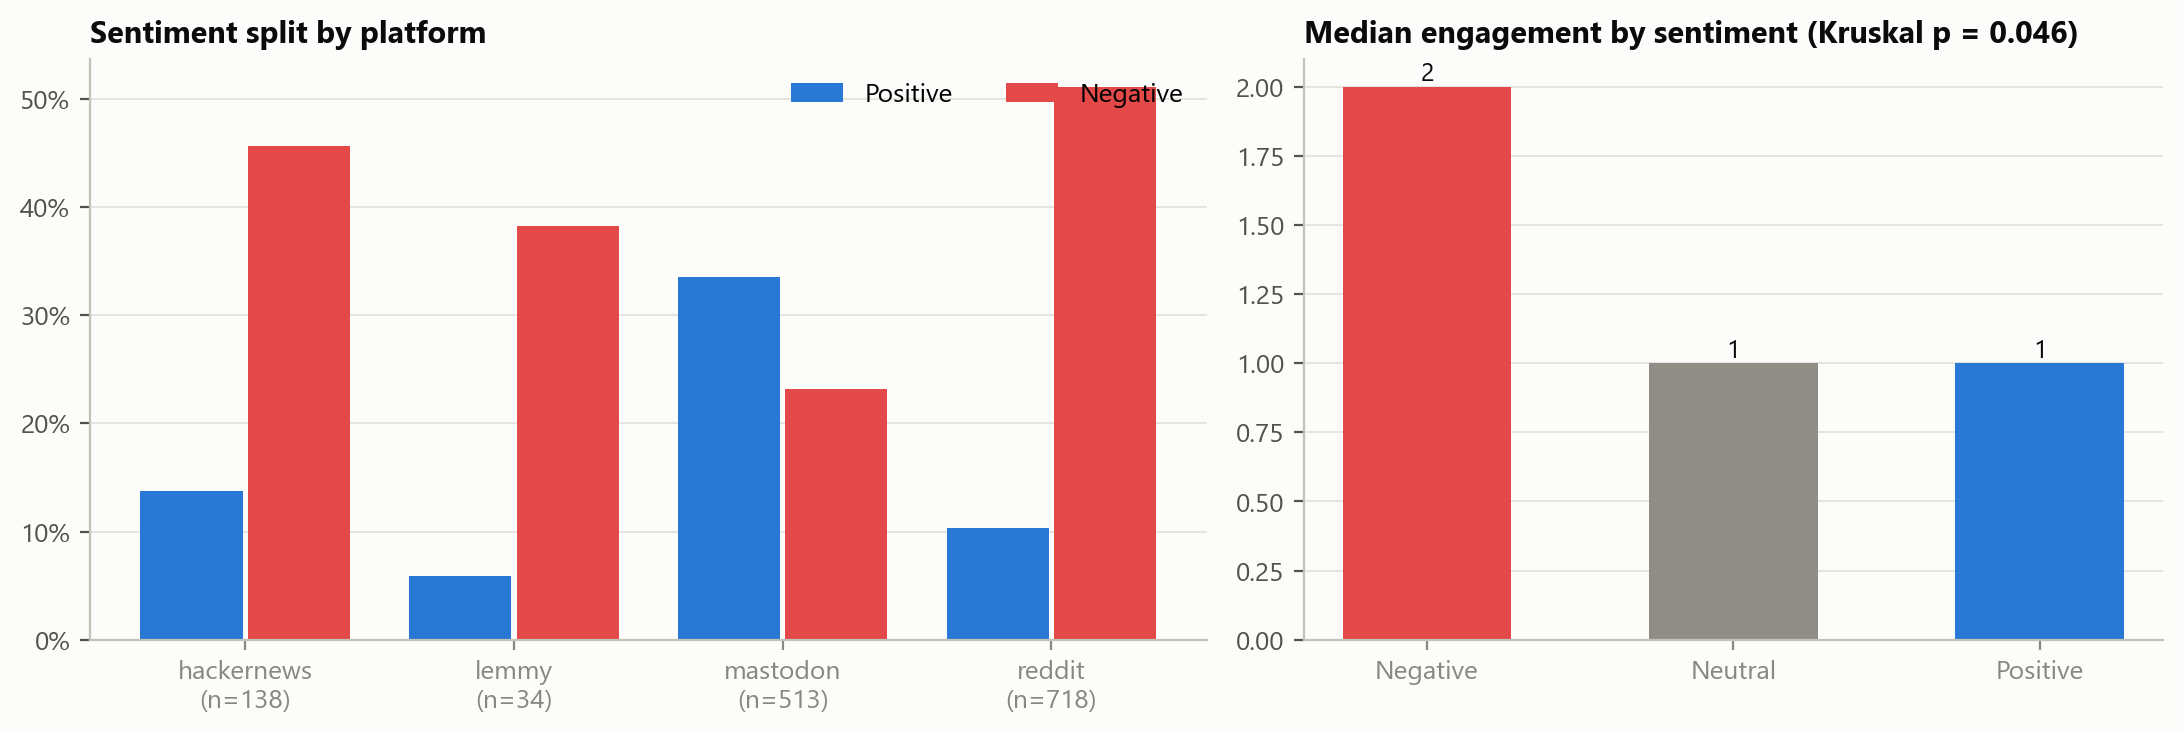
\includegraphics[width=\textwidth]{Entropy_r3_platform_engagement.png}
\caption{Sentiment split by platform, and median engagement by sentiment class.}
\end{figure}

The gap is explainable rather than mysterious: Mastodon hashtag timelines carry announcements and enthusiast posts, whereas the subreddits searched here are where people go \emph{to ask for help}, so their baseline is complaints. \textbf{Negative posts also earn more engagement} (median 2 versus 1 for neutral and positive, Kruskal--Wallis $p = 0.046$, n = 584) -- the same ``outrage engagement'' pattern measured in Round 1.

\section{Real-time behaviour}

The pipeline is not a single snapshot. The collector ran twice, every row records the moment it was fetched, and the second run added \textbf{233 posts} to the analysis set (110 Negative, 91 Neutral, 32 Positive), moving the newest tracked post from 09:33 to 10:44 UTC. A live refresh executed at the end of the notebook then pulled a further \textbf{17 posts} published after the dataset was saved and scored them with the same model (9 Neutral, 6 Negative, 2 Positive), confirming the loop runs continuously rather than once.

\section{Robustness checks and baselines}

Four checks were run against the claims above, each interrogating a specific way this analysis could be wrong. They live in \texttt{Entropy\_03\_robustness\_checks.py} and write \texttt{outputs/Entropy\_round3\_robustness.json}.

\subsection{Is the decline a pile-on by a few accounts?}

The most economical explanation for any measured drop in sentiment is that a small number of accounts posted a large number of complaints. It is not what happened here. The analysis set holds \textbf{1403 posts from 1132 distinct authors} (1.24 posts per author), and 87\% of those authors appear exactly once. The busiest single account contributes 18 posts and the ten busiest together account for only 5.6\% of the corpus. Restricting to negative posts alone, \textbf{562 negative posts come from 521 distinct authors} -- barely more than one apiece -- with the ten busiest contributing 5.2\%. The shift reflects many people reacting independently, not a campaign.

\subsection{Does the model beat an off-the-shelf tool?}

A reused fine-tuned ensemble is only worth its complexity if it beats something anyone could install in a minute. VADER, a rule-based lexicon scorer built for social media text, was run over the same 150 hand-labelled posts with its standard $\pm 0.05$ compound thresholds.

\begin{table}[H]
\centering\small
\begin{tabular}{@{}lrr@{}}
\toprule
\textbf{Scorer} & \textbf{Macro-F1} & \textbf{Accuracy} \\
\midrule
VADER lexicon (baseline) & 0.496 & --- \\
Round 2 ensemble, as-is & 0.712 & --- \\
\textbf{Round 2 ensemble, chunked $+$ neutral bias} & \textbf{0.699} & \textbf{0.707} \\
\bottomrule
\end{tabular}
\caption{All three scored against the same 140-post human consensus. The reused ensemble beats the lexicon baseline by 0.203 macro-F1.}
\end{table}

The gap is large enough to justify the transfer: at 0.496 macro-F1 VADER is close to chance on three balanced classes, largely because it reads technical complaint language as neutral. The domain shift that costs our model 0.06 against its own test set still leaves it far ahead of the obvious alternative.

\subsection{Would a monitoring rule have caught this?}

Analysing a launch after it is over is not monitoring. To test whether this pipeline would have been useful in real time, a deliberately simple rule was replayed over the window: \emph{net sentiment <= -0.15 for 2 consecutive 12h bins with n >= 20}.

The rule first fires at \textbf{2026-09-15 12:00 UTC}, \textbf{19 hours after release}, and it raises \textbf{0 false alarms} in the pre-launch period. A team watching this dashboard would have known the reception had turned within a day, while the press coverage was still reporting the redesign.

\begin{figure}[H]
\centering
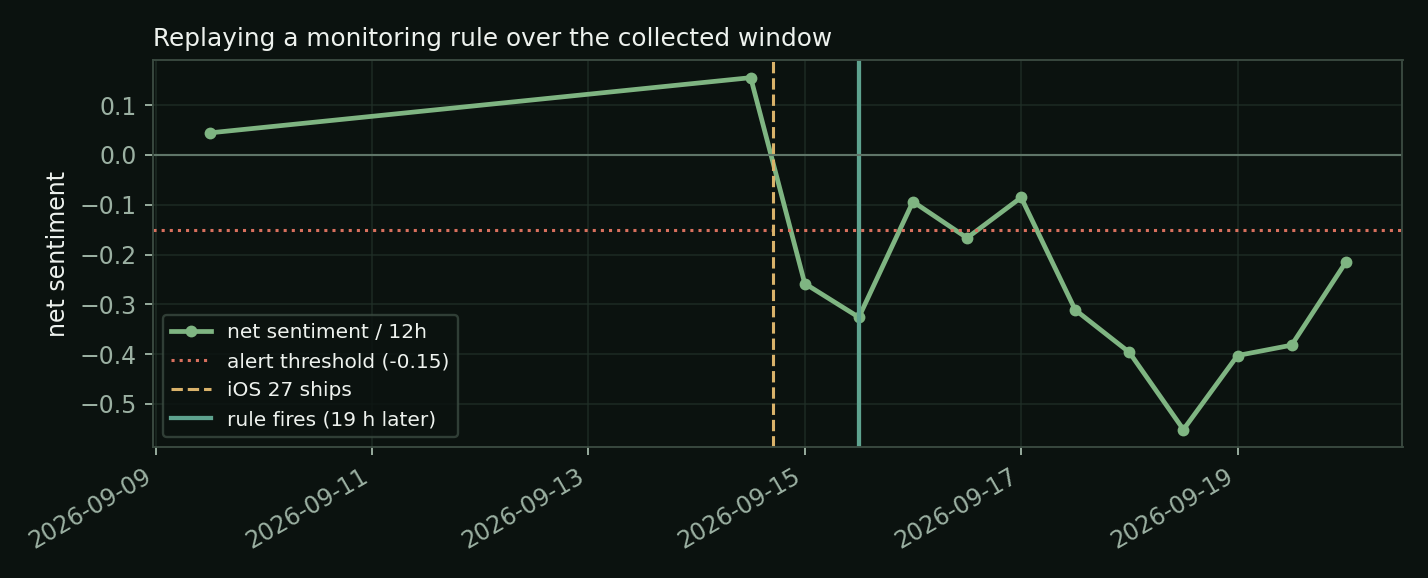
\includegraphics[width=0.94\textwidth]{Entropy_r3_fig9_alerting.png}
\caption{The alerting rule replayed over the collected window. The threshold is crossed decisively after release and never before it.}
\end{figure}

\subsection{Inter-annotator agreement}

The original 150 labels came from a single annotator, which was the weakest methodological point in this round. Both team members then labelled the same 150 posts independently, from a shuffled sheet with the model's predictions and the first annotator's labels removed.

\begin{itemize}[leftmargin=*]
  \item \textbf{Cohen's $\kappa$ = 0.896} between the two annotators over all 150 posts (93.3\% raw agreement), which is `almost perfect' agreement on the conventional scale.
  \item The 140 posts they agree on become the \textbf{reference standard} for every accuracy figure in this report. The 10 they disagree on are set aside rather than adjudicated, so no tie is broken by the people being measured.
  \item Each annotator agrees with the original single-annotator labels at only $\kappa \approx 0.64$--$0.66$, well below their agreement with each other. That gap is the reason the consensus replaced the original labels rather than supplementing them.
  \item The consensus set is also better balanced: 35 Positive posts against the 15 in the original sample, so the Positive-class score is no longer resting on a handful of examples.
\end{itemize}

\section{Limitations}

\begin{itemize}[leftmargin=*]
  \item \textbf{No Reddit engagement.} The RSS interface omits scores, so engagement analysis rests on Hacker News, Mastodon and Lemmy (584 scored posts).
  \item \textbf{Platform mix is not constant} across the window, which inflates the raw decline; section 4.5 is the correction, not a footnote.
  \item \textbf{Model accuracy in this domain is 0.699 macro-F1}, below the 0.723 measured on tweets, and the interval remains wide because 140 posts is a small validation set with only 15 Positive examples. Reported \emph{levels} are noisier than reported \emph{changes}.
  \item \textbf{Validation labels are our own.} Both team members labelled the 150 posts independently ($\kappa = 0.896$) and only the 140 they agreed on are used, but they remain our judgements rather than an external gold standard.
  \item \textbf{English-only and public-only.} Non-English posts are excluded, and X, TikTok and YouTube are out of reach without paid API access.
  \item \textbf{Keyword recall.} A post reacting to the update without naming it is not in the analysis set.
\end{itemize}

\section{Conclusion}

The monitoring layer works end to end: it collected live public reaction with no paid APIs, scored it with the Round 2 model, and located the moment opinion turned, with statistical support and named causes.

For this release the story is that \textbf{a launch that began in indifference soured within three days, and reliability, not design, did the damage}. The baseline was never measurably positive -- what the data supports is a fall from neutral, and that fall is large, significant, spread across 521 distinct authors, and detectable by a simple rule within 19 hours. If Apple were reading this dashboard, the queue would be the PWA regression, macOS application compatibility, notification behaviour, and the distance between Apple Intelligence marketing and its reception. The redesign, which absorbed most of the press coverage, is the thing people mind least.

Two methodological lessons carry beyond this dataset. First, \textbf{a single global sentiment line is misleading} when the source mix moves; per-platform baselines are mandatory, and negative content is amplified by engagement on every platform we measured. Second, \textbf{a model must be validated in the domain where it is deployed}: reusing the Round 2 ensemble unchanged was correct, but its accuracy here is six points lower than its training-domain score, and two inference details -- an unapplied operating point and silent truncation of two thirds of the corpus -- were worth more than any modelling change.

\end{document}
